\documentclass[ignorenonframetext,10pt,aspectratio=169]{beamer}

\usepackage{umut}
\usepackage{umuttr}
\usepackage[utf8]{inputenc}
\usepackage{uling}
\usepackage{natbib,unatbib}
\usepackage{linguex}
         \renewcommand{\refdash}{}
\usepackage{ubeamer}
\usepackage{verbatim}

\usepackage{tikz-qtree}
\usetikzlibrary{er,positioning}

\title{Alternation Rules by FSTs}
\author{\  \\ \vspace{20pt} Umut \"Ozge\\  }

\date{COGS 532: Theoretical Linguistics\\ METU, Informatics}

\begin{document}

\begin{frame}\frametitle{}
\thispagestyle{empty}
\maketitle
\end{frame}

\begin{frame}[t,plain]
\end{frame}

\begin{frame}[t,plain]
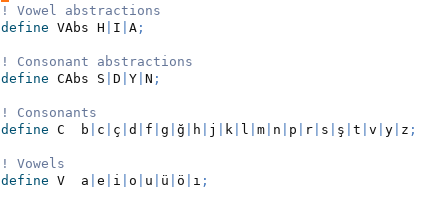
\includegraphics[scale=0.4]{img/img1.png}
\end{frame}

\begin{frame}[t,plain]
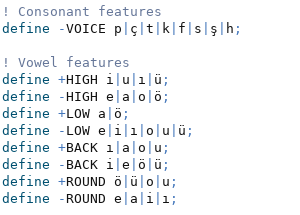
\includegraphics[scale=0.4]{img/img2.png}
\end{frame}
\begin{frame}[t,plain]
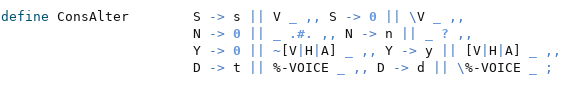
\includegraphics[scale=0.4]{img/img3.png}
\end{frame}
\begin{frame}[t,plain]
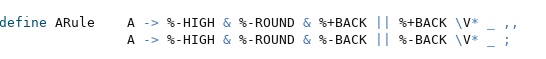
\includegraphics[scale=0.4]{img/img4.png}
\end{frame}
\begin{frame}[t,plain]
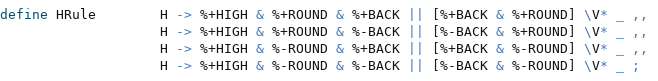
\includegraphics[scale=0.4]{img/img5.png}
\end{frame}
\begin{frame}[t,plain]
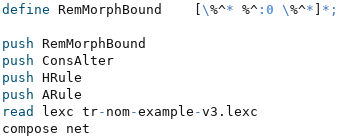
\includegraphics[scale=0.4]{img/img6.png}
\end{frame}
\begin{frame}[t,plain]

\end{frame}

\begin{frame}[t,plain]

\end{frame}

\begin{frame}[t,plain]

\end{frame}

\begin{frame}[t,plain]

\end{frame}
\end{document}
